\input{../common/head.tex}
\def\passYear{2016}
\def\faculty{физико-технический институт}
\def\department{Кафедра информационной безопасности}
\def\departmentHead{Н. В. Грайворонский}
\def\kind{Дипломна робота}
\def\level{магістр}
\def\specialityCode{8.04030101}
\def\specialityTitle{Прикладная математика}
\def\theme{Структуры для работы с большими объёмами данных в Python}
\def\gender{female}
\def\mentorGender{male}
\def\course{2}
\def\group{ФИ-41}
\def\name{Лавягина Ольга Алексеевна}
\def\mentorRank{}
\def\mentorName{Колотий Андрей Всеволодович}
\def\reviewerRank{Rank}
\def\reviewerName{Name}
\def\subject{Специальные разделы программирования}


\usepackage{csvsimple}

\begin{document}

\import{1_title/}{title.tex}

\clearpage

\pagenumbering{gobble}
%\import{3_abstract/}{main.tex}

%\pagestyle{empty}
%\thispagestyle{empty}
%\tableofcontents

\clearpage
\pagenumbering{arabic}
\pagestyle{fancy}
\setcounter{page}{2}

\clearpage

\chapter{Данные}

Материалы для лабораторной работы были получены на геопортале геологической служды США --- USGS \cite{USGS}. Скачанный архив содержит каналы изображений. Каждое изображение космических аппаратов (КА) серии Landsat имеет уникальный идентификатор, структура которого следующая:

[Идентификатор сенсора и КА (3 символа)] + [Координаты снимка в WRS-2-системе (Path, Row, 6 символов)] + [Год] + [DOY] + [Режим съёмки (5 символов)].

Например, LC81810252015048LGN00 --- снимок КА Landsat-8, полученный сенсором OLI/TIRS; координаты снимка в системе WRS-2 --- 818 (Path) 102 (Row), съёмка проведена 48-го дня 2015 года, режим съёмки LGN00. Содержание архива с продуктом уровня обработки  данного снимка изображено на рисунке \ref{archive}. 

\begin{figure}[h]
  \centering
  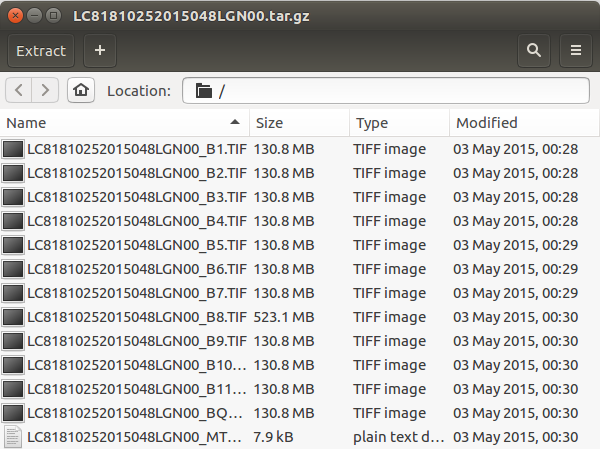
\includegraphics[width=.75\textwidth]{archive.png}
  \caption{Архив с продуктом обработки дынных КА Landsat-8 OLI/TIRS уробня обратотки L1T}
\label{archive}
\end{figure}


\chapter{Задание}

Средствами командной строки операционной чистемы, а также с помощью бинариев библиотеки GDAL разработать автоматический сценарий, который будет совершать обработку данных дистанционного зондирования Земли (ДЗЗ), соответственнос поставленными заданиями.

Задание 1. Распаковка набора архивов с продуктами ДЗЗ в новосозданные папки, названия которых будут соответствовать идентификаторам изображения.

Задание 2. Конкатинация каналов видимого, ближнего и среднего инфракрасного спектрального диапазонов изображения в единственный GEOTIFF файл.

Задание 3. Перепроектирование спутникового изображения в указанную картографическую систему координат.

Задание 4. Конкатинация изображений двух соседних <<row>> с одинаковым <<path>>.

Задание 5. Обрезка результирующего изображения по заданному векторному контуру.

Ход выполнения работы. Получить архивы с сутниковыми изображениями, и файл с векторным контуром для дальнейшей обрезки. Средствами командной строки операционной системы (без ограничения в выборе ОС) и с использованием бинариев библиотеуи GDAL создать программный сценарий для автоматической обработки спутниковых изображений согласно поставленным заданиям. 

\chapter{Листинг кода}


\chapter*{Выводы}
\addcontentsline{toc}{chapter}{Выводы}

\clearpage
\phantomsection
\addcontentsline{toc}{chapter}{Список литературы}
\renewcommand\bibname{Список литературы}
\bibliography{bibliography.bib}

\end{document}
